\documentclass[12pt]{article}
\usepackage{graphicx}
  
%
% Title[Enter title of the experiment here]
\title{EE230: Experiment No.9\\
Instrumentation amplifier on load cell \\
Sensor}

% Author[Enter details of author here]
\author{Mudavath vishnuvardhan,200070044}

% begin the document.
\begin{document}

% make a title page.[this creates title page]
\maketitle

%\textbf{ * All experiment reports may not contain all fields in this format,This document is just for your reference*} 

\section{Overview of the experiment} %[This segment creates Section as seen in document]

\subsection{Aim of the experiment}%[This segment creates sebsections under the same section]

The experiment aims at familiarizing the student with the implementation of
an instrumentation amplifier to amplify output from a load cell sensor by
creating the circuit on a breadboard and applying known weights to the
weighing machine to generate inputs.

\subsection{Methods}
To attain the objectives listed, a circuit was developed on a breadboard using
provided circuit diagrams which was hooked up to a weighing machine and
known weights were applied to it to achieve required voltage values.
Additionally gain in terms of mV/gm was computed to get a sense of the
sensitivity of the amplifier.


\section{Design}%[To add multiple sections, keep appending blocks like this]
Due to the deformation in the load, the modified resistance values are :
\begin{equation}
R_{a}=R_{g}+\Delta R
\end{equation}  
\begin{equation}
R_{b}=R_{g}-\Delta R
\end{equation}  
\begin{equation}
R_{c}=R_{g}-\Delta R
\end{equation}  
\begin{equation}
R_{d}=R_{g}+\Delta R\\
 \end{equation}  
 Due to this the output voltage of the load cell snesor is \(V_{out+}\) and \(V_{out-}\)
 \begin{equation}
V_{out+}=(R_{g}+\Delta R )*(V_{in+}-V_{in-})/ (2R_{g})
\end{equation} 
\begin{equation} 
V_{out-}=(R_{g}-\Delta R )*(V_{in+}-V_{in-})/ (2R_{g})
\end{equation} 
\begin{equation}
V_{out+}+V_{out-}=(\Delta R )*(V_{in+}-V_{in-})/ (2R_{g})\\
 \end{equation}  
\subsection{Instrumentation Amplifier using TL084 IC}
A Instrumentation Amplifier was designed using using TL084 IC. The
amplifiers were run on ±12V supply voltage. To obtain a gain of 300, the
values of the resistances were chosen as follows:
\begin{equation}
A_{v}=R_{4}/R_{3}(1+2R_{2}/R_{1})
 \end{equation}  
 \begin{figure}
\centering
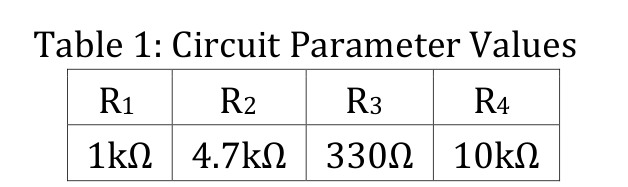
\includegraphics[scale = 0.3]{table1.png}
\end{figure}
Furthermore the load cell sensor was set up for providing input to the 3
opamp Instrumentation Amplifier. A ±5V supply and ground for bridge was
given to the weighing machine and the raw load cell output was connected
to the input of the instrumentation amplifier. The circuit diagram for the
same has been attached below :
\newpage
\begin{figure}
\centering
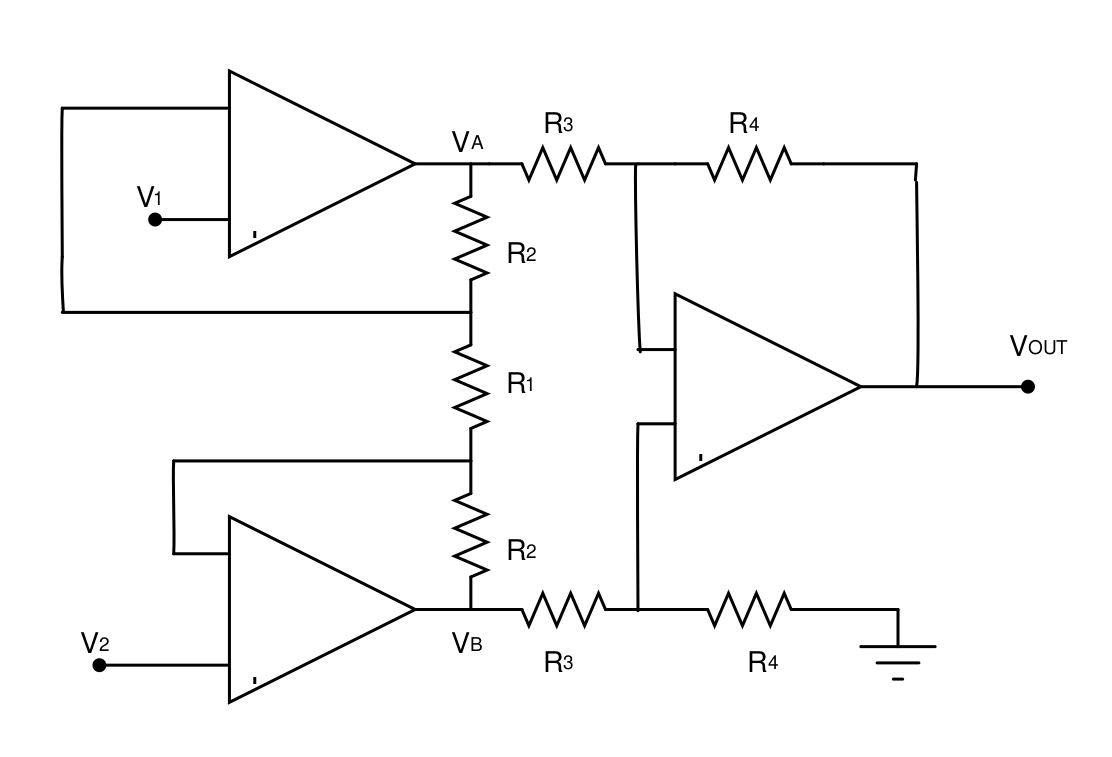
\includegraphics[scale = 0.3]{ins_amp_tl084.png}
\end{figure}
\subsection{Instrumentation Amplifier using 1NA128 IC}
A Instrumentation Amplifier was designed using using INA128 Amplifier.
The amplifiers were run on ±12V supply voltage. The parameters of the
circuit were : Furthermore the load cell sensor was set up for providing input
\begin{figure}
\centering
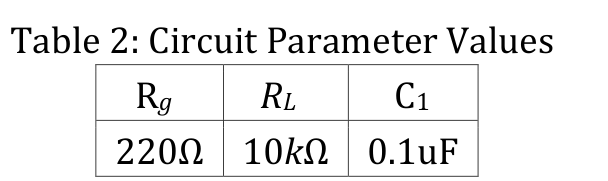
\includegraphics[scale = 0.3]{table2.png}
\end{figure}
to the 3 op-amp Instrumentation Amplifier. A ±5V supply and ground for
bridge was given to the weighing machine and the raw load cell output was
connected to the input of the instrumentation amplifier. The circuit diagram
for the same has been attached below :
\newpage
\begin{figure}
\centering
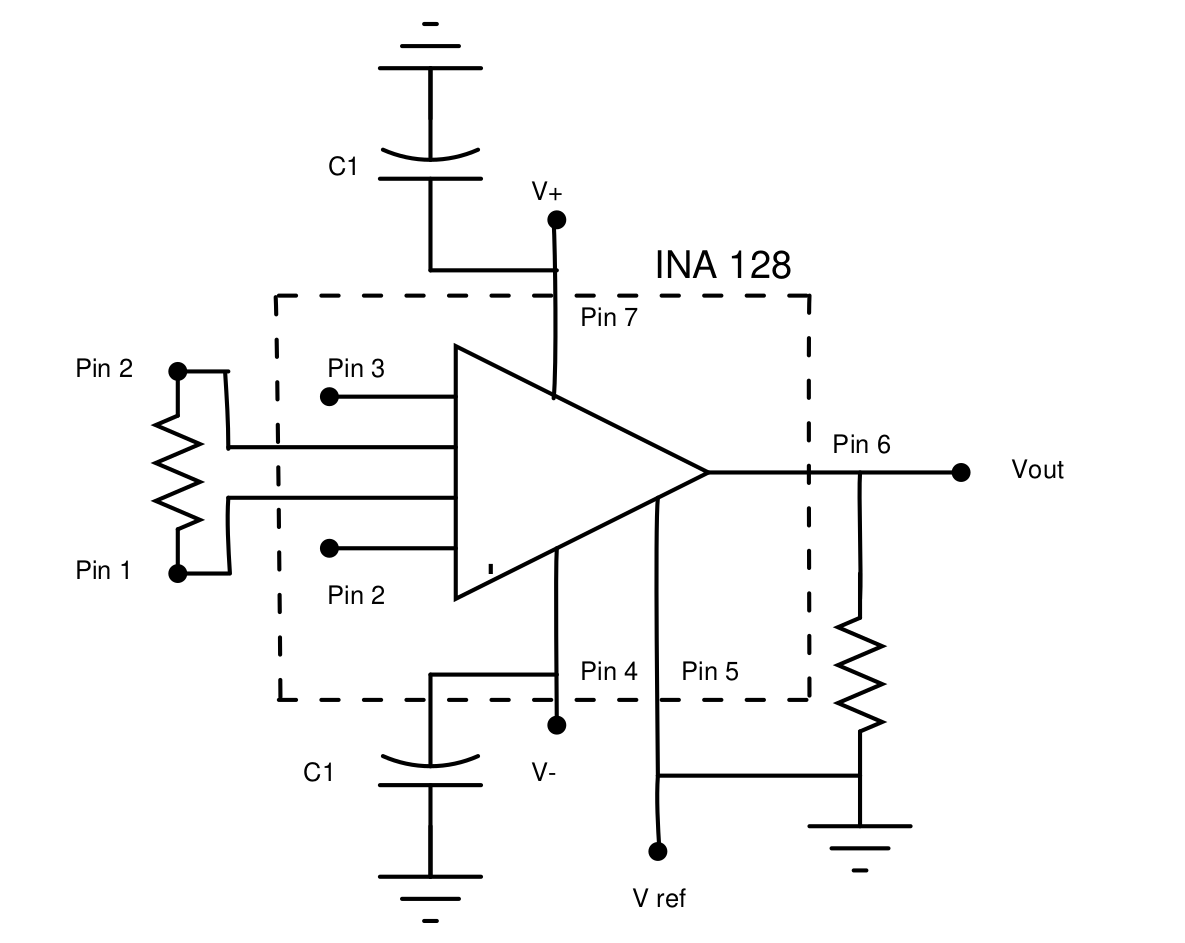
\includegraphics[scale = 0.3]{ins_amp_1na128.png}
\end{figure}


\section{Experimental results}
\subsection{Instrumentation Amplifier using TL084 IC}
The circuit was designed to provide a gain of 300. When the circuit was
connected to the load cell sensor and the output was plotted for varying
amount of weights, the relationship of Vout vs weight looked like : Based on
readings obtained from graph, the obtained value of the sensitivity in mV/gm
was 2.55.
\begin{figure}
\centering
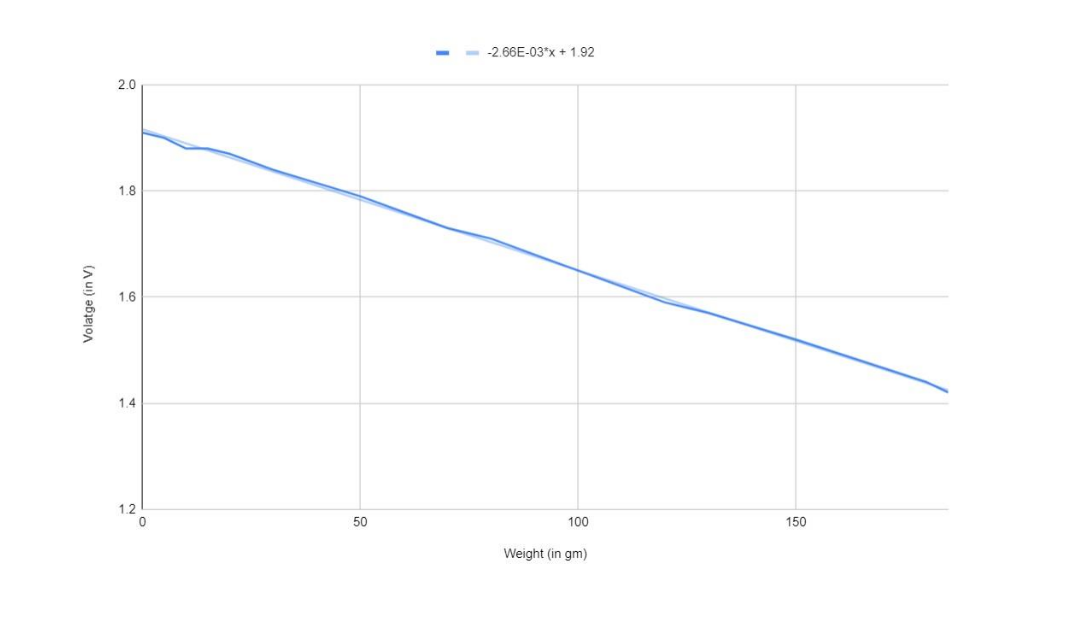
\includegraphics[scale = 0.4]{graph1.png}
\end{figure}
\newpage
\subsection{Instrumentation Amplifier using 1NA128 IC}
When the circuit was connected to the load cell sensor and the output was
plotted for varying amount of weights, the relationship of Vout vs weight
looked like :
Based on readings obtained from graph, the obtained value of the sensitivity
in mV/gm was 0.171.
\begin{figure}
\centering
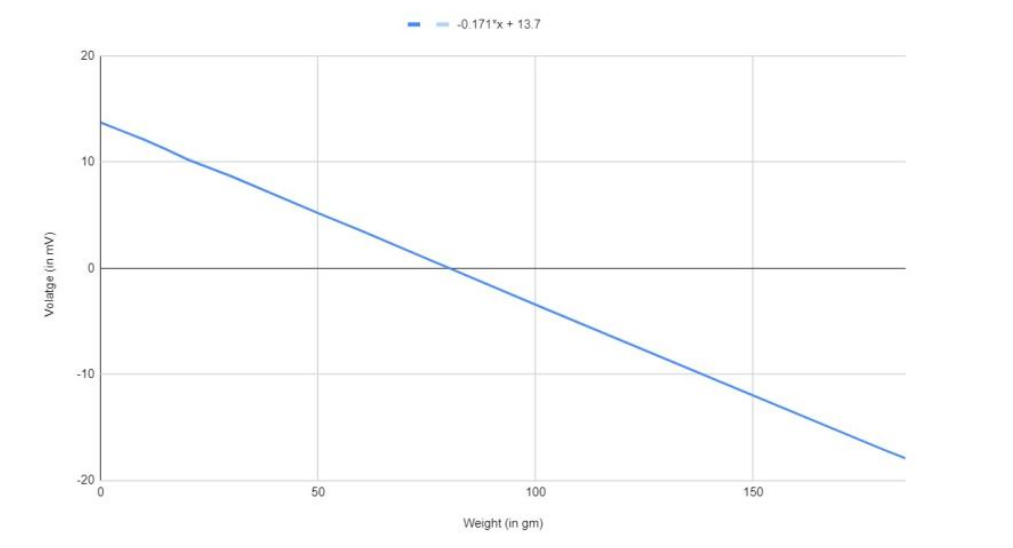
\includegraphics[scale = 0.4]{graph2.png}
\end{figure}
\newpage
Upon halving the value of Rg to get double the sensitivity, the modified plot
and sensitivity were 0.34.
\begin{figure}
\centering
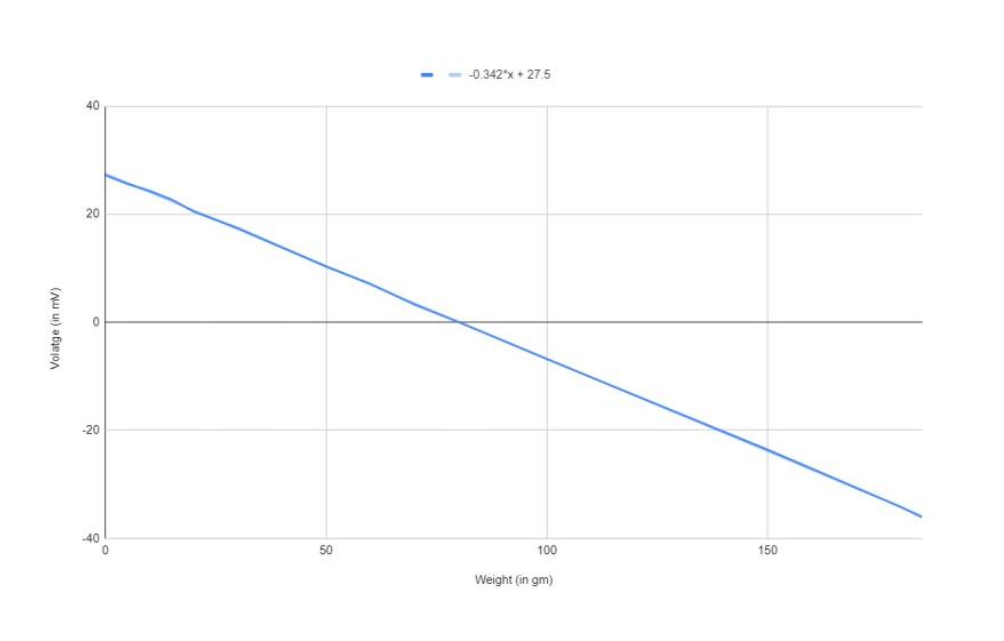
\includegraphics[scale = 0.4]{graph3.png}
\end{figure}
\newpage
\section{Experiment completion status}
I have completed all parts of the experiment in lab only.

\end{document}
